\documentclass[a4paper]{article}
\usepackage[utf8]{inputenc}
\usepackage[warn]{mathtext}
\usepackage[russian]{babel}

\usepackage{natbib}

\usepackage{caption}
\usepackage{graphicx}
\graphicspath{}
\DeclareGraphicsExtensions{.pdf,.png,.jpg}
\DeclareSymbolFont{T2Aletters}{T2A}{cmr}{m}{it}
\usepackage{subcaption}

\usepackage{csvsimple}

\begin{document}
\begin{minipage}{0.8\textwidth}
\begin{center}
    \large{Санкт-Петербургский национальный исследовательский университет информационных технологий, механики и оптики
\\УЧЕБНЫЙ ЦЕНТР ОБЩЕЙ ФИЗИКИ ФТФ}
\medbreak
\end{center}
\end{minipage}
\hfill
\begin{minipage}{0.3\textwidth}

\includegraphics[scale=0.4]{itmo.jpg}
\end{minipage}

\noindent\rule{\textwidth}{1pt}
\medbreak
\begin{minipage}{0.5\textwidth}
Группа $\textit{P3112}$						
\\Студент $\textit{Сенина Мария Михайловна}$			
\\Преподаватель $\textit{Сорокина Е К}$
\end{minipage}
\hfill
\begin{minipage}{0.4\textwidth}
К работе допущен
\\Работа выполнена
\end{minipage}

\bigbreak

\begin{center}
        \Large{\textbf{Рабочий протокол и отчёт по лабораторной работе 2-04}}
   \LARGE{\textbf{\\Определение вязкости жидкости}}
\end{center}

\section{Цель работы}
Определить коэффициент вязкости масла.

\section{Задачи, решаемые при выполнении работы}
\begin{enumerate}
    \item Определить коэффициент внутреннего трения касторового
масла методом Стокса.
    \item Проверка справедливости формулы Стокса для шариков
разного диаметра.
\end{enumerate}

\section{Объект исслевдования}
Масло в сосуде.

\section{Метод экспериментального исследования}
В жидкостях и некоторых газах величина силы внутреннего трения между слоями, возникающего при движении одних слоёв относительно других пропорциональна площади слоёв $\Delta S$и градиенту их скорости $\frac{d v}{dx}$. Коэффициент этой пропорциональности - $\eta$. Т.е. $F = \eta \frac{dv}{dx} \Delta S$. $\eta$ - коэффициент вязксти жидкости и зависит от физических свойств данной жидкости и её температуры.

Этот коэффициент можно определить исходя из закона Стокса - если шарик движется в жидкости с постоянной скоростью сила трения в жидкости будет ровна $F = 6\pi\eta v r$. Сделав поправку на то, что мы будем ронять дробинки не в бесконечной жидкости, а в целиндрическом сосуде можно получить следующую зависимость: $F = \frac{6\pi \eta v r}{k}$,  где $k$ - та сама поправка, $k = \frac{1}{1 + \frac{2.4 r}{R}}$,  где $r$ радиус шарика, а $R$ - радиус сосуда.

Т.к. скорость шарика постоянна на него действует нулевое ускорение. Значит $F_{тр} + F_a= mg$, откуда можно выразить коэффициент вязкости $\eta = \frac{9}{2}\frac{r^2(\rho_ш - \rho_ж)}{v} k g$.

Таким образом мы можем посчитать значение $\eta$, измерив раадиус шарика на микроскопе, радиус целиндра, расстояние, которое шарик проходит с неизменной скоростью и засекая время, за которое он это сделает.

\section{Рабочие формулы}
\begin{enumerate}
    \item Среднее значение  $\frac{\sum_{i=1}^n x_i}{n} $
    \item Закон Стокса: зависимость силы трения от скорости $F = \frac{6\pi \eta v r}{k}$
    \item $k = \frac{1}{1 + \frac{2.4 r}{R}}$ - поправка для закона Стокса, для шарика движущегося в целиндрическом сосуде
    \item Коэффициент вязкости $\eta = \frac{9}{2}\frac{r^2(\rho_ш - \rho_ж)}{v} k g$.
    \item Погрешность коэффициента вязкости $\Delta \eta =  \eta \sqrt{(2\frac{\Delta r}{r})^2 + (\frac{\Delta v}{v})^2 + (\frac{\Delta g}{g})^2 + \frac{(\Delta \rho_ш)^2 - (\Delta \rho_ж)^2}{(\rho_ш - \rho_ж)^2}}$
    \item Диаметр дробинки $d = \overline{d} = \frac{\sum_{i=1}^N (x_{2i} - x_{1i})}{N}$
    \item Радиус дробинки $r = \frac{d \alpha}{2}$, где $\alpha$ - погрешность микроскопа
    \item Погрешность радиуса дробинки $\Delta r = (\frac{\Delta d}{d} + \frac{\Delta \alpha}{\alpha})r$
    \item Скорость $v = \frac{l}{t}$
    \item Погрешность скорости $\Delta v =  \sqrt{(\frac{\Delta l}{l})^2 (\frac{\Delta t}{t})^2}$
    \item Погрешность измерений через коэффицент Стьюденса $\Delta x = t_{a_{дов, N}}\sqrt{\frac{\sum\limits_{i=1}^N (x - \bar{x})^2}{N (N-1)}}$, где $t_{a_{дов, N}}$ - коэффицент Стьюдентса для доверительной вероятности $a_{дов}$ и количества измерений $N$.
\end{enumerate}
\section{Измерительные приборы}
$\textbf{Погрешности измерительных приборов}$

\begin{tabular}{ l | l | l | l }\hline
№ & Наименование & Используемый диапазон & Погрешность прибора \\ \hline
1 & Микроскоп  &  $(0.9 - 1.9 ) 10^{-3}$ мм  & $ 1 10^{-3} $ мм \\  \hline
2 &	Секундомер & 6.32 - 26.5 с & 	0,01 с \\   \hline
\end{tabular}

\section{Схема установки}

\begin{figure}[h!]
\begin{minipage}[h]{0.49\linewidth}
\center{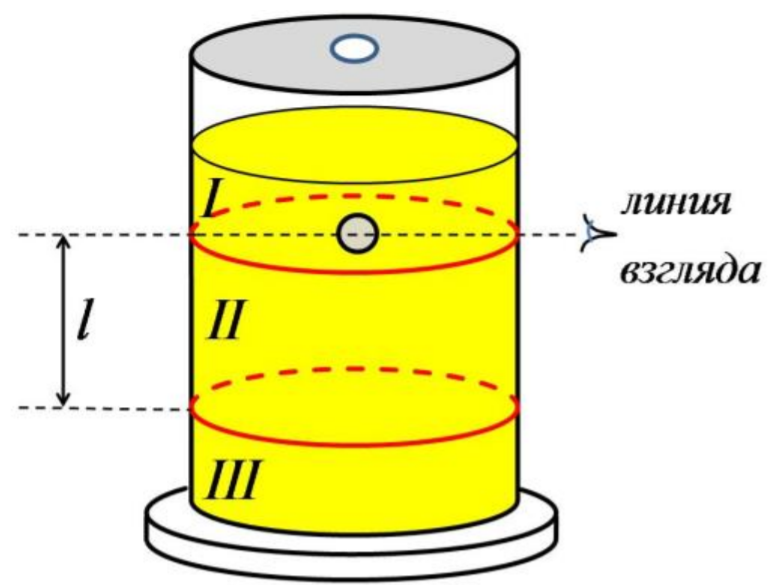
\includegraphics[width=0.5\linewidth]{stend1.png} \\ а) колба с маслом}
\end{minipage}
\hfill
\begin{minipage}[h]{0.49\linewidth}
\center{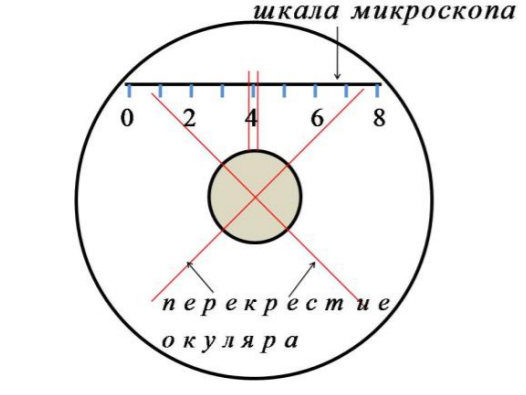
\includegraphics[width=0.5\linewidth]{stend2.png} \\ б) вид шкалы в микроскопе}
\end{minipage}
\caption{Стенд}
\label{stend}
\end{figure}


$\textbf{Параметры стенда}$\\
\begin{tabular}{l | l | l | l }\hline
№ & Наименование & Значение & Погрешность \\ \hline
1 & Радиус колбы $R$ & 2.95 см & 0.05 см \\
2 & Плотность шарика $\rho_ш$ & 7.8 $\frac{г}{см^3}$ & 0.1 $\frac{г}{см^3}$ \\
3 & Плотность масла $\rho_м$ & 0.96 $\frac{г}{см^3}$ & 0.04 $\frac{г}{см^3}$ \\
4 & Цена деления микроскопа $\alpha$ & 0.266 $\frac{мм}{дел}$ & 0.001 $\frac{мм}{дел}$ \\
5 & Расстояние, которое проходит шарик $l$ & 10 см & 0.5 см \\
\end{tabular}

\section{Результаты прямых измерений}
См. в приожении 1

\section{Расчёт результатов косвенных измерений}
Для каждой таблицы по формулам $d = \overline{d} = \frac{\sum_{i=1}^N (x_{2i} - x_{1i})}{N}$ (6) и $\Delta r = (\frac{\Delta d}{d} + \frac{\Delta \alpha}{\alpha})r$ (11) я вычислила диаметр каждой дробинки. Оказалось, что две из трёх дробинок, которые мне дали оказались одного размера с точностью до погрешности, а третья дробинка была в два раза меньше первых двух:

\begin{enumerate}
    \item $d_1 = 3.57 \ дел$ и $\Delta d_1 = 0.04 \ дел$ 
    \item $d_2 = 7.43 \ дел$ и $\Delta d_2 = 0.06 \ дел$
    \item $d_3 = 7.47 \ дел$ и $\Delta d_3 = 0.05 \ дел$
\end{enumerate}

Далее по формулам $r = \frac{d \alpha}{2}$ и $\Delta r = (\frac{\Delta d}{d} + \frac{\Delta \alpha}{\alpha})r$ я посчитала значения радиусов дробинок:

\begin{enumerate}
    \item $r_1 = \frac{3.57 \ дел \ 266 \cdot 10^{-3} \ м/дел}{2} = 475 \cdot 10^{-6} \ м$ и $\Delta r_1 = (\frac{0.04 \ дел}{3.57 \ дел} + \frac{1 \cdot 10^{-3} \ м/дел}{266 \cdot 10^{-3} \ м/дел}) \cdot 475 \cdot 10^{-6} = 5 \cdot 10^{-6} \ м$
    \item $r_1 = \frac{7.43 \ дел \ 266 \cdot 10^{-3} \ м/дел}{2} = 988 \cdot 10^{-6} \ м$ и $\Delta r_1 = (\frac{0.06 \ дел}{7.43 \ дел} + \frac{1 \cdot 10^{-3} \ м/дел}{266 \cdot 10^{-3} \ м/дел}) \cdot 988 \cdot 10^{-6} = 9 \cdot 10^{-6} \ м$
    
    \item $r_1 = \frac{7.47 \ дел \ 266 \cdot 10^{-3} \ м/дел}{2} = 994 \cdot 10^{-6} \ м$ и $\Delta r_1 = (\frac{0.05 \ дел}{7.47 \ дел} + \frac{1 \cdot 10^{-3} \ м/дел}{266 \cdot 10^{-3} \ м/дел}) \cdot 994 \cdot 10^{-6} = 7 \cdot 10^{-6} \ м$
\end{enumerate}

Зная, время, за которое каждый шарик прошёл расстояние $l = 10$ см, по формулам $v = \frac{l}{t}$ и $\Delta v =  \sqrt{(\frac{\Delta l}{l})^2 (\frac{\Delta t}{t})^2}$ я посчитала скорости шариков:

\begin{enumerate}
    \item $v_1 = \frac{0.1 \ м}{26.5 \ с} = 38 \cdot 10^{-4} \frac{м}{c}$, $\Delta v = \sqrt{(\frac{0.005 \ м}{0.1 \ м})^2 (\frac{\Delta 0.01 \ c}{26.5 \ c})^2} = 2 \cdot 10^{-4} \frac{м}{c}$
    \item $v_1 = \frac{0.1 \ м}{6.72 \ с} = 149 \cdot 10^{-4} \frac{м}{c}$, $\Delta v =\sqrt{(\frac{0.005 \ м}{0.1 \ м})^2 (\frac{\Delta 0.01 \ c}{6.72 \ c})^2} = 7 \cdot 10^{-4} \frac{м}{c}$
    \item $v_1 = \frac{0.1 \ м}{6.32 \ с} = 158 \cdot 10^{-4} \frac{м}{c}$, $\Delta v =\sqrt{(\frac{0.005 \ м}{0.1 \ м})^2 (\frac{\Delta 0.01 \ c}{6.32 \ c})^2} = 7 \cdot 10^{-4} \frac{м}{c}$
\end{enumerate}

А по формулам $\eta = \frac{9}{2}\frac{r^2(\rho_ш - \rho_ж)}{v} k g$, где $k = \frac{1}{1 + \frac{2.4 r}{R}}$ и $\Delta \eta =  \eta \sqrt{(2\frac{\Delta r}{r})^2 + (\frac{\Delta v}{v})^2 + (\frac{\Delta g}{g})^2 + \frac{(\Delta \rho_ш)^2 - (\Delta \rho_ж)^2}{(\rho_ш - \rho_ж)^2}}$ я посчитала $\eta$ и его погрешность:

\begin{enumerate}
    \item $\eta_1 = \frac{9}{2}\frac{(475 \cdot 10^{-6} \ м)^2(7800 \ кг/м^3 - 960 \ кг/м^3)}{38  \cdot 10^{-4} \ м/c}\cdot \frac{1}{1 + \frac{2.4 \cdot 475 \dot 10^{-6} \ м}{29.5 \cdot 10^{-3} м}} \cdot 9.82 \ м/c^2 = 858  \cdot 10^{-3} \ Па \cdot c$
    
    $\Delta \eta_1 = 858  \cdot 10^{-3}  \ Па \cdot c \sqrt{(2\frac{5 \cdot 10^{-6} \ м}{475 \cdot 10^{-6} \ м})^2 + (\frac{2 \cdot 10^{-4} \ м/c}{38 \cdot 10^{-4} \ м/c})^2 + \frac{(100 \ кг/м^3)^2 - (40 \ кг/м^3)^2}{(7800 \ кг/м^3 - 960 \ кг/м^3)^2}} = 48 \cdot 10^{-3} Па \cdot с$
    
    \item $\eta_2 = \frac{9}{2}\frac{(988 \cdot 10^{-6} \ м)^2(7800 \ кг/м^3 - 960 \ кг/м^3)}{149  \cdot 10^{-4} \ м/c}\cdot \frac{1}{1 + \frac{2.4 \cdot 988 \dot 10^{-6} \ м}{29.5 \cdot 10^{-3} м}} \cdot 9.82 \ м/c^2 = 907 \ Па \cdot c$
    
    $\Delta \eta_1 = 907  \cdot 10^{-3}  \ Па \cdot c \sqrt{(2\frac{9 \cdot10^{-6} \ м}{988  \cdot 10^{-6} \ м})^2 + (\frac{7 \cdot 10^{-4} \ м/c}{149 \cdot 10^{-4} \ м/c})^2 + \frac{(100 \ кг/м^3)^2 - (40 \ кг/м^3)^2}{(7800 \ кг/м^3 - 960 \ кг/м^3)^2}} = 50 \cdot 10^{-3} Па \cdot с$
    
    \item $\eta_3 = \frac{9}{2}\frac{(994 \cdot 10^{-6} \ м)^2(7800 \ кг/м^3 - 960 \ кг/м^3)}{158  \cdot 10^{-4} \ м/c}\cdot \frac{1}{1 + \frac{2.4 \cdot 994 \dot 10^{-6} \ м}{29.5 \cdot 10^{-3} м}} \cdot 9.82 \ м/c^2 = 862  \cdot 10^{-3} \ Па \cdot c$
    
    $\Delta \eta_1 = 862  \cdot 10^{-3}  \ Па \cdot c \sqrt{(2\frac{7 \cdot 10^{-6} \ м}{994 \cdot 10^{-6} \ м})^2 + (\frac{7 \cdot 10^{-4} \ м/c}{158 \cdot 10^{-4} \ м/c})^2 + \frac{(100 \ кг/м^3)^2 - (40 \ кг/м^3)^2}{(7800 \ кг/м^3 - 960 \ кг/м^3)^2}} = 46 \cdot 10^{-3} Па \cdot с$
\end{enumerate}

Получается, что: 
\begin{enumerate}
    \item $\eta_1 = (858 \pm 48) \cdot 10^{-3} \ Па \cdot c$
    \item $\eta_2 = (907 \pm 50) \cdot 10^{-3} \ Па \cdot c$
    \item $\eta_3 = (862 \pm 46) \cdot 10^{-3} \ Па \cdot c$
\end{enumerate}

\section{ Окончательные результаты}
 $\eta = (876 \pm 81 ) 10^{-3} Па \cdot с$
 \\ $\delta \eta = 0.09$

\section{Выводы}
Я нашла коэффициент внутреннего трения касторового масла методом Стокса с точностью до 9\%.
Проведя это эксперимет я выяснила, что размер шарика не влияет на результат эксперимента. Хотя два из трёх моих шариков были одинакового размера, так что результаты можно улучшить, проведя повторное исследование с другим размером шаров.
\end{document}